\documentclass[12pt]{article}
\usepackage[a4paper, margin=2cm]{geometry}
\usepackage[english]{babel} % To obtain English text with the blindtext package
\usepackage{blindtext}
\usepackage{graphicx} % Required for inserting images
\usepackage{array, multirow} % For extra column formatting
\usepackage{amsmath, amssymb, cancel} %for equation environment
\usepackage{float}
\usepackage{parskip} % For gaps between para
\usepackage{setspace}
\usepackage{pdfpages}
\usepackage{abstract}
\usepackage[export]{adjustbox}
\usepackage{emptypage}
\usepackage{tocloft}
\usepackage[nottoc]{tocbibind}
\usepackage{hyperref, url}
\usepackage[table]{xcolor}
\usepackage{minted}
    \usemintedstyle{monokai}
\usepackage{caption,subcaption}
    \captionsetup{font=footnotesize,labelfont=bf}
    \subcaptionsetup{font=footnotesize}
\usepackage{tcolorbox}
    \newtcolorbox{mintedbox}{
        colback=backcolour,
        boxrule=0pt,
        sharp corners,
        width=\linewidth,
        left=0pt, right=0pt,
        top=3pt, bottom=3pt
    }
\usepackage{cite,wrapfig}

\cftsetindents{section}{0em}{2em}
\cftsetindents{subsection}{0em}{2em}

\renewcommand\cfttoctitlefont{\hfill\Large\bfseries}
\renewcommand\cftaftertoctitle{\hfill\mbox{}}

\graphicspath{ {./images/} }

\definecolor{blurple}{HTML}{5865F2}
\definecolor{backcolour}{HTML}{272823}

\hypersetup{
    colorlinks=true,
    linkcolor=black,
    urlcolor=black,
    citecolor=blurple,
}

\urlstyle{same}

\pagenumbering{arabic}

\renewcommand{\arraystretch}{1.3}

\setcounter{secnumdepth}{5}
\setcounter{tocdepth}{5}
\newcommand\simpleparagraph[1]{%
  \stepcounter{paragraph}\paragraph*{\theparagraph\quad{}#1}}

%%%%%%%%%%%%%%%%%%%%%%%%%%%%%%%%%%%


\title{PHYC20080 Exp.5 Oscilloscope}
\author{Joana Adao}
\date{\today}

\begin{document}

\begin{titlepage}
    \begin{center}

        \begin{figure}[ht]
            
\includegraphics[width=\textwidth]{UCDLogo.png}
        \end{figure}
        
        \begin{figure}
            \centerline{
\includegraphics[width=\paperwidth]{UCDBanner.png}}
        \end{figure}

        \vspace{4cm}

        {\LARGE \bfseries PHYC20080 Fields, Waves and Light}\\
        \vspace{0.75cm}
        {\Large Experiment No.5 Studying Sound Using an Oscilloscope}
        
        \vspace{1cm}
    
    {\Large \textbf{8 April 2025}}
    
    \vspace{2cm}
    
    {\large \textbf{by Joana C.C. Adao (Student No. 23311051)}}\\
    \vspace{.25cm}
    {\large With Beau Etac}\\
    \vspace{0.25cm}
    {\large Tuesday 16.00-18.00 Slot}\\
    {\large Chiara (Coordinator)}

    \end{center}
    
   \clearpage

\end{titlepage}

\begin{center}
    \section*{Abstract}
    \addtocontents{toc}{\protect\contentsline{section}{\textbf{Abstract}}{\hfill}{}}
    \thispagestyle{empty}
\end{center}

The aim of this experiment was to determine the speed of sound with the use of an oscilloscope through two investigations. 

Investigation I focused on resonant waves in a closed tube
at constant frequencies for varying tube lengths. The following relationship for the wavelength in a closed tube, $\lambda = \tfrac{4}{n}L$ was used, and in turn used in the relationship $c=f\lambda$ to
determine the speed of sound in air. This yielded the values of \textbf{286.02 m/s} $\mathbf{\pm}$ \textbf{25.62 m/s} for 700 Hz, \textbf{319.68 m/s} $\mathbf{\pm}$ \textbf{17.92 m/s} for 800 Hz,
\textbf{270.36 m/s} $\mathbf{\pm}$ \textbf{24.21 m/s} for 900 Hz, and \textbf{267.40 m/s} $\mathbf{\pm}$ \textbf{28.50 m/s} for 1000 Hz. These values were consistently lower than the expected value of 343 m/s for room temperature,
which indicates measurement errors like errors in determining peak resonant amplitude and possible parallax when measuring tube length.

Investigation II made use of square wave sound pulses and echo time difference to calculate the speed of sound via $c = \tfrac{2L}{\Delta t}$. The average speed of sound measured using this method was found to be
\textbf{348.71 m/s} $\mathbf{\pm}$ \textbf{5.678 m/s}. This value is quite close to the expected value of 343 m/s at room temperature, and the fact that the value is slightly higher than what is expected at 20$^{\circ}$C suggest the room at the time of
measuring was warmer. This method of measuring the speed of sound may result in higher accuracy in comparison to the previous investigation.

\newpage

\tableofcontents
\thispagestyle{empty}

\newpage

%%%%%%%%%%%%%%%%%%%%%%%%%%%%%%%%%%%

\setcounter{page}{1}
\section{Theory} \label{sec:1}

\subsection{Waves}

\textbf{Transverse waves} travel in a series of peaks and troughs with \textit{perpendicular} vibration to the motion. These are the kinds of physical waves seen when water ripples \cite{waveffden}.
\textbf{Longitudinal waves} vibrate \textit{parallel} to the motion. Instead of peaks and troughs there are areas of compression, in which molecules get pushed together, and
areas of rarefraction, in which molecules are pulled away and spaced out \cite{waveffden,studywave,acousticsound}. Sound waves are longitudinal waves, and the speed of sound can be calculated when the wavelength and frequency and source are known \cite{UCDoscilloscope}:

\vspace{-2ex}
\begin{gather} \label{eq:1}
    v = f \lambda
\end{gather}

where $v$ is the speed (of sound, in this case), $f$ is the frequency, and $\lambda$ is the wavelength.

\subsection{Resonance}

Resonance is a phenomenon in which an object will vibrate with more strength when an external oscillation passes through it and matches the object's natural frequency \cite{resbrit,reslibre}.
In a tube, resonant standing waves that travel in each direction can be created, which differ based on the tube structure and corresponding displacement of air (see Figure \ref{fig:1}) \cite{tuberes}.

\begin{figure}[H]
    \centering
    \begin{subfigure}[b]{.45\textwidth}
        \centering
        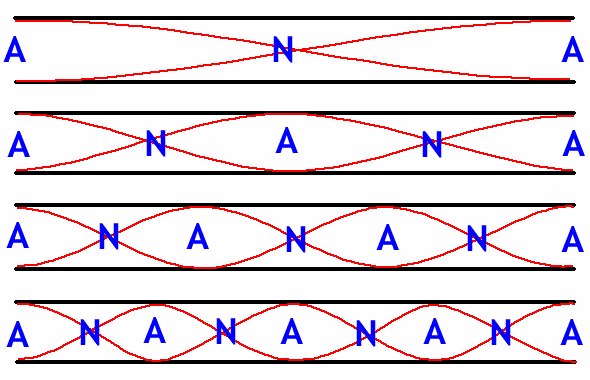
\includegraphics[width=\linewidth]{open resonance.png}
        \caption{\centering Tube open at both ends.}
        \label{fig:1a}
    \end{subfigure}
    \hfill
    \begin{subfigure}[b]{.45\textwidth}
        \centering
        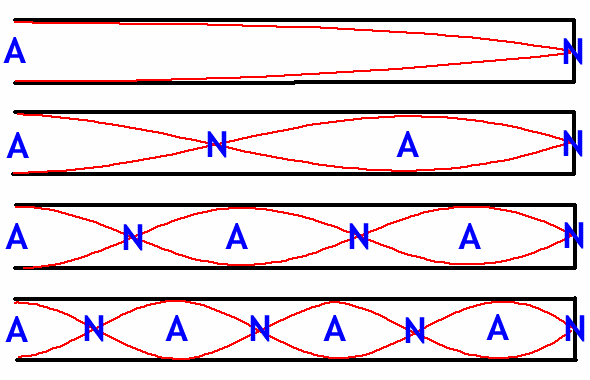
\includegraphics[width=\linewidth]{closed resonance.png}
        \caption{\centering Tube open at one end.}
        \label{fig:1b}
    \end{subfigure}
    \caption{Standing waves patterns for the first four resonances in a tube open at both ends (\subref{fig:1a}) and a tube open at one end (\subref{fig:1b}). Nodes ("N") and anti-nodes ("A")
    are labelled \protect\cite{openclosedres}.}
    \label{fig:1}
\end{figure}

For completely \textbf{open tubes} the air can move freely between both sides, and so there will be a displacement anti-node of maximum frequency at each end (see Figure \ref{fig:1a}, A) \cite{tuberes}.
The harmonics, places of resonance, of an open tube occur exactly as it would on a string with the following formula \cite{UCDoscilloscope,tuberes},

\vspace{-2ex}
\begin{gather}
    \lambda_n = \frac{2}{n}L \qquad\qquad n=1,2,3,4 \dotsc
\end{gather}

where $n$ is an integer, $L$ is the tube length, and $\lambda$ is the wavelength.

For \textbf{closed tubes} with only one end open air cannot move as freely considering one of the ends is closed, at which there will always be a node of the lowest possible wavelength (see Figure \ref{fig:1b}, N) \cite{tuberes}.
The harmonics of a closed tube can be considered as being half of what was seen for open tubes (better visualised in Figure \ref{fig:1}), and so the formula reads \cite{UCDoscilloscope,tuberes},

\vspace{-2ex}
\begin{gather} \label{eq:3}
    \lambda_n = \frac{4}{n}L \qquad\qquad n=1,2,3,4 \dotsc
\end{gather}

where $n$ is an integer, $L$ is the tube length, and $\lambda$ is the wavelength once again.

\subsection{The Oscilloscope}

Oscilloscopes are devices that can visually display electrical signals as waves, typically sine waves, in order to show the variations of that electrical signal over time
\cite{flukeoscillo,keyoscillo,oscil101}. It allows for the measurements of period, frequency, and voltage through a grid of divisions \cite{oscil101}.

\begin{figure}[H]
    \centering
    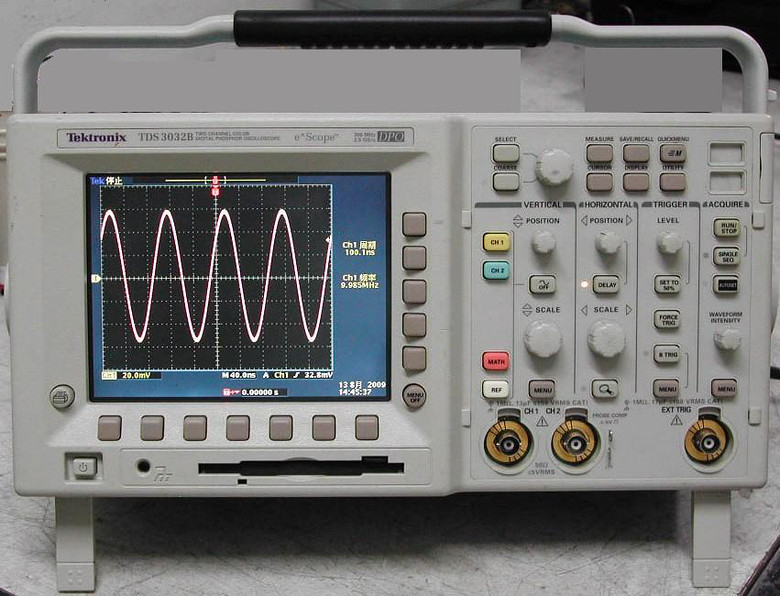
\includegraphics[width=.6\textwidth]{tektronix tds3052.jpg}
    \caption{\centering \footnotesize{Tektronix TDS 3052 Oscillospce with 2 channels, showing a sine wave and divisions clearly visible \protect\cite{tektronixtds3052}}}
    \label{fig:2}
\end{figure}

For analogue oscilloscopes like the one in Figure \ref{fig:2} that make use of phosphor screens, beams of electrons from the electrical signals are what draw the waveforms on up to 2 channels \cite{oscil101}.
Knobs allow for the changing of the vertical gain (Volts per division) and horizontal sweep (time per division) without changing the signal itself \cite{UCDoscilloscope,oscil101}.
The trigger button is what allows for smoother reading, where the oscilloscope only captures a signal when it crosses certain voltages \cite{oscil101}.

\newpage

\section{Methodology} \label{sec:2}

The apparatus used throughout this experiment was set up as per Figure \ref{fig:3} and two different investigations were carried out.

\begin{figure}[H]
    \centering
    \begin{subfigure}[b]{.49\textwidth}
        \centering
        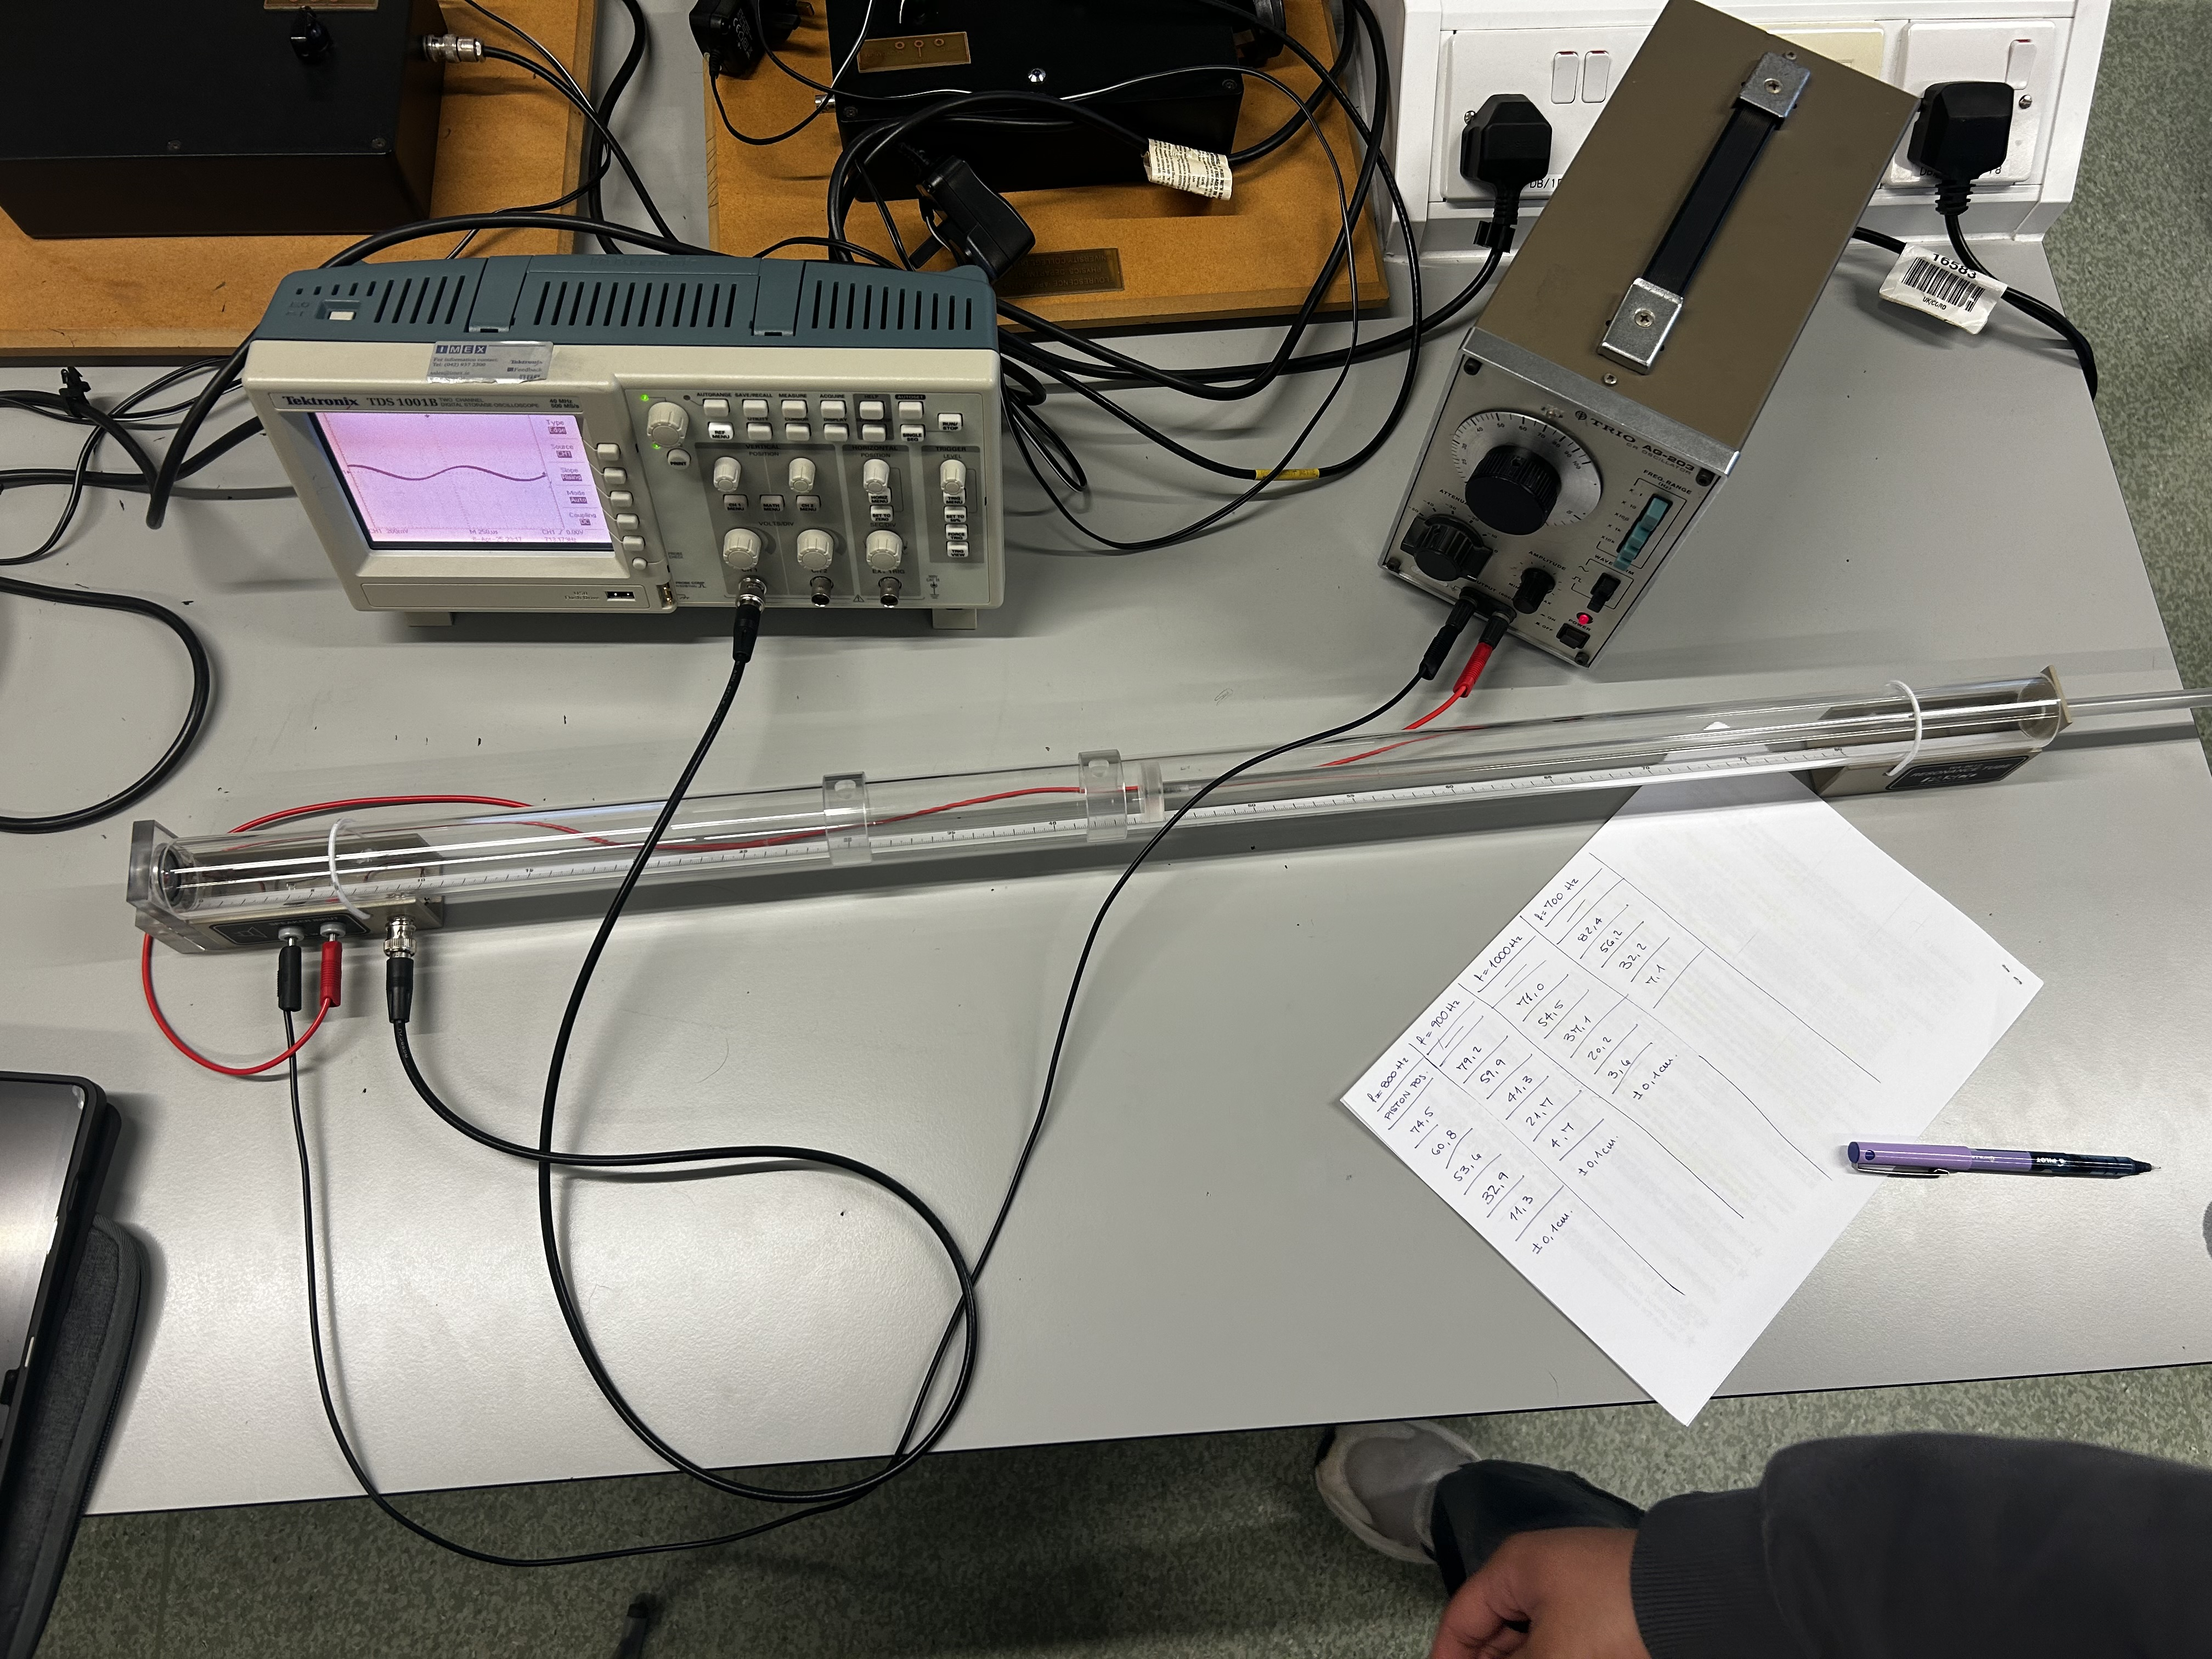
\includegraphics[width=\linewidth]{exp oscil setup.jpeg}
    \end{subfigure}
    \hfill
    \begin{subfigure}[b]{.49\textwidth}
        \centering
        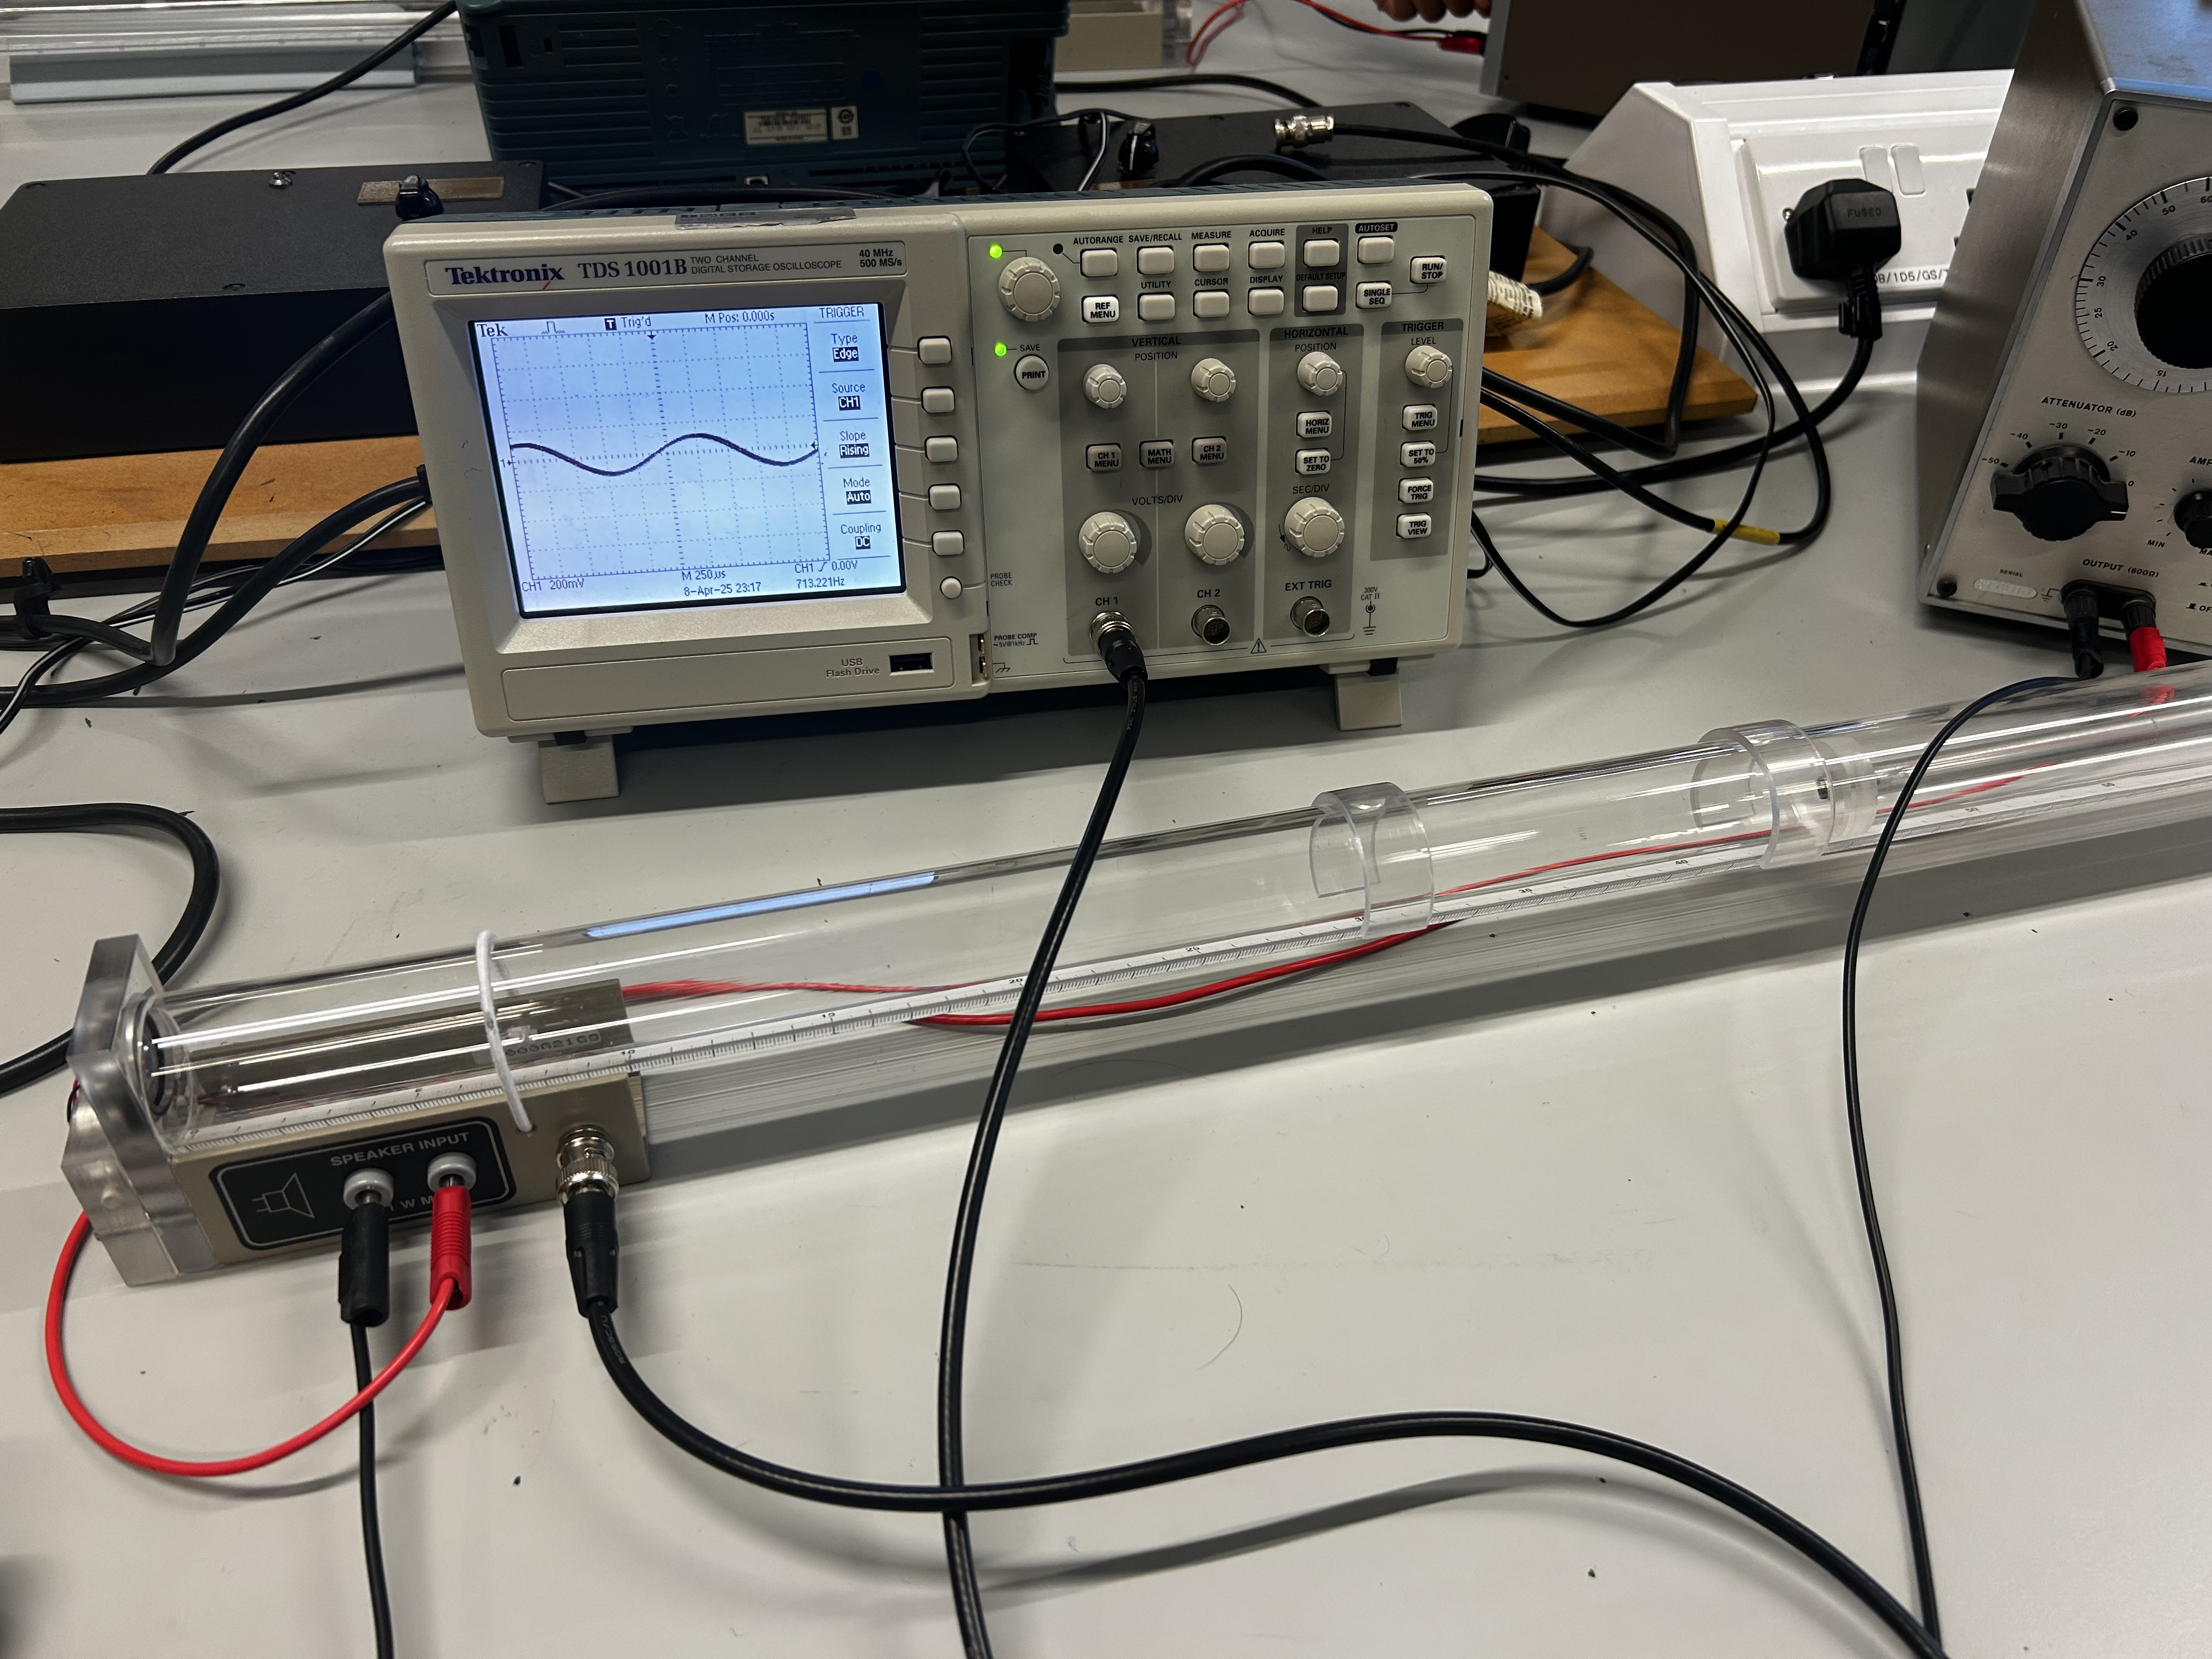
\includegraphics[width=\linewidth]{exp oscil oscil.jpeg}
    \end{subfigure}
    \caption{Experimental setup of the tube, plunger, and oscilloscope.}
    \label{fig:3}
\end{figure}

\subsection{Investigation I}

This section of the experiment investigated resonant frequencies at different tube lengths of a closed tube, varied by the plunger piston for constant frequencies.
The microphone connected to the oscilloscope measured the resonant frequency in the tube as the length varied, but it was very sensitive to outside sounds. To help counteract this, the oscilloscope was set to an automatically-decided trigger, forming a smooth, legible wave.
By having a stable wave, the maximum resonant frequency was easily seen on the oscilloscope display and recorded. The lowest resonant frequency was also easily seen as the wave became unstable.

The amplitude was turned up suitably, loud enough to be heard without blowing the speaker. Higher amplitudes meant for more defined waves on the oscilloscope. Distance measurements were taken for each point of highest resonant frequency as seen on the oscilloscope for all resonant positions.
This procedure was then repeated for at least 3 other frequencies. These measurements are then used in tandem with Eq. \ref{eq:1} to calculate the speed of sound in air.

\subsection{Investigation II}

This section of the experiment investigated pulses of sound at a constant frequency of \textbf{10 Hz} as square waves as they propagated through set tube lengths and then were reflected.
The speaker made a distinct clicking sound as the sound waves were produced when amplitude was set to a reasonable amount. The oscilloscope output will appear as Figure \ref{fig:4} and the time separation between the initial pulse to the first echo (first two largest pulses on the display) was measured through
the horizontal time divisions. As for Figure \ref{fig:4}, it can be read at the bottom of the entire grid that each time division is 2.50 ms. The tube length was varied for 5 lengths, each time separation recorded.

\begin{figure}[H]
    \centering
    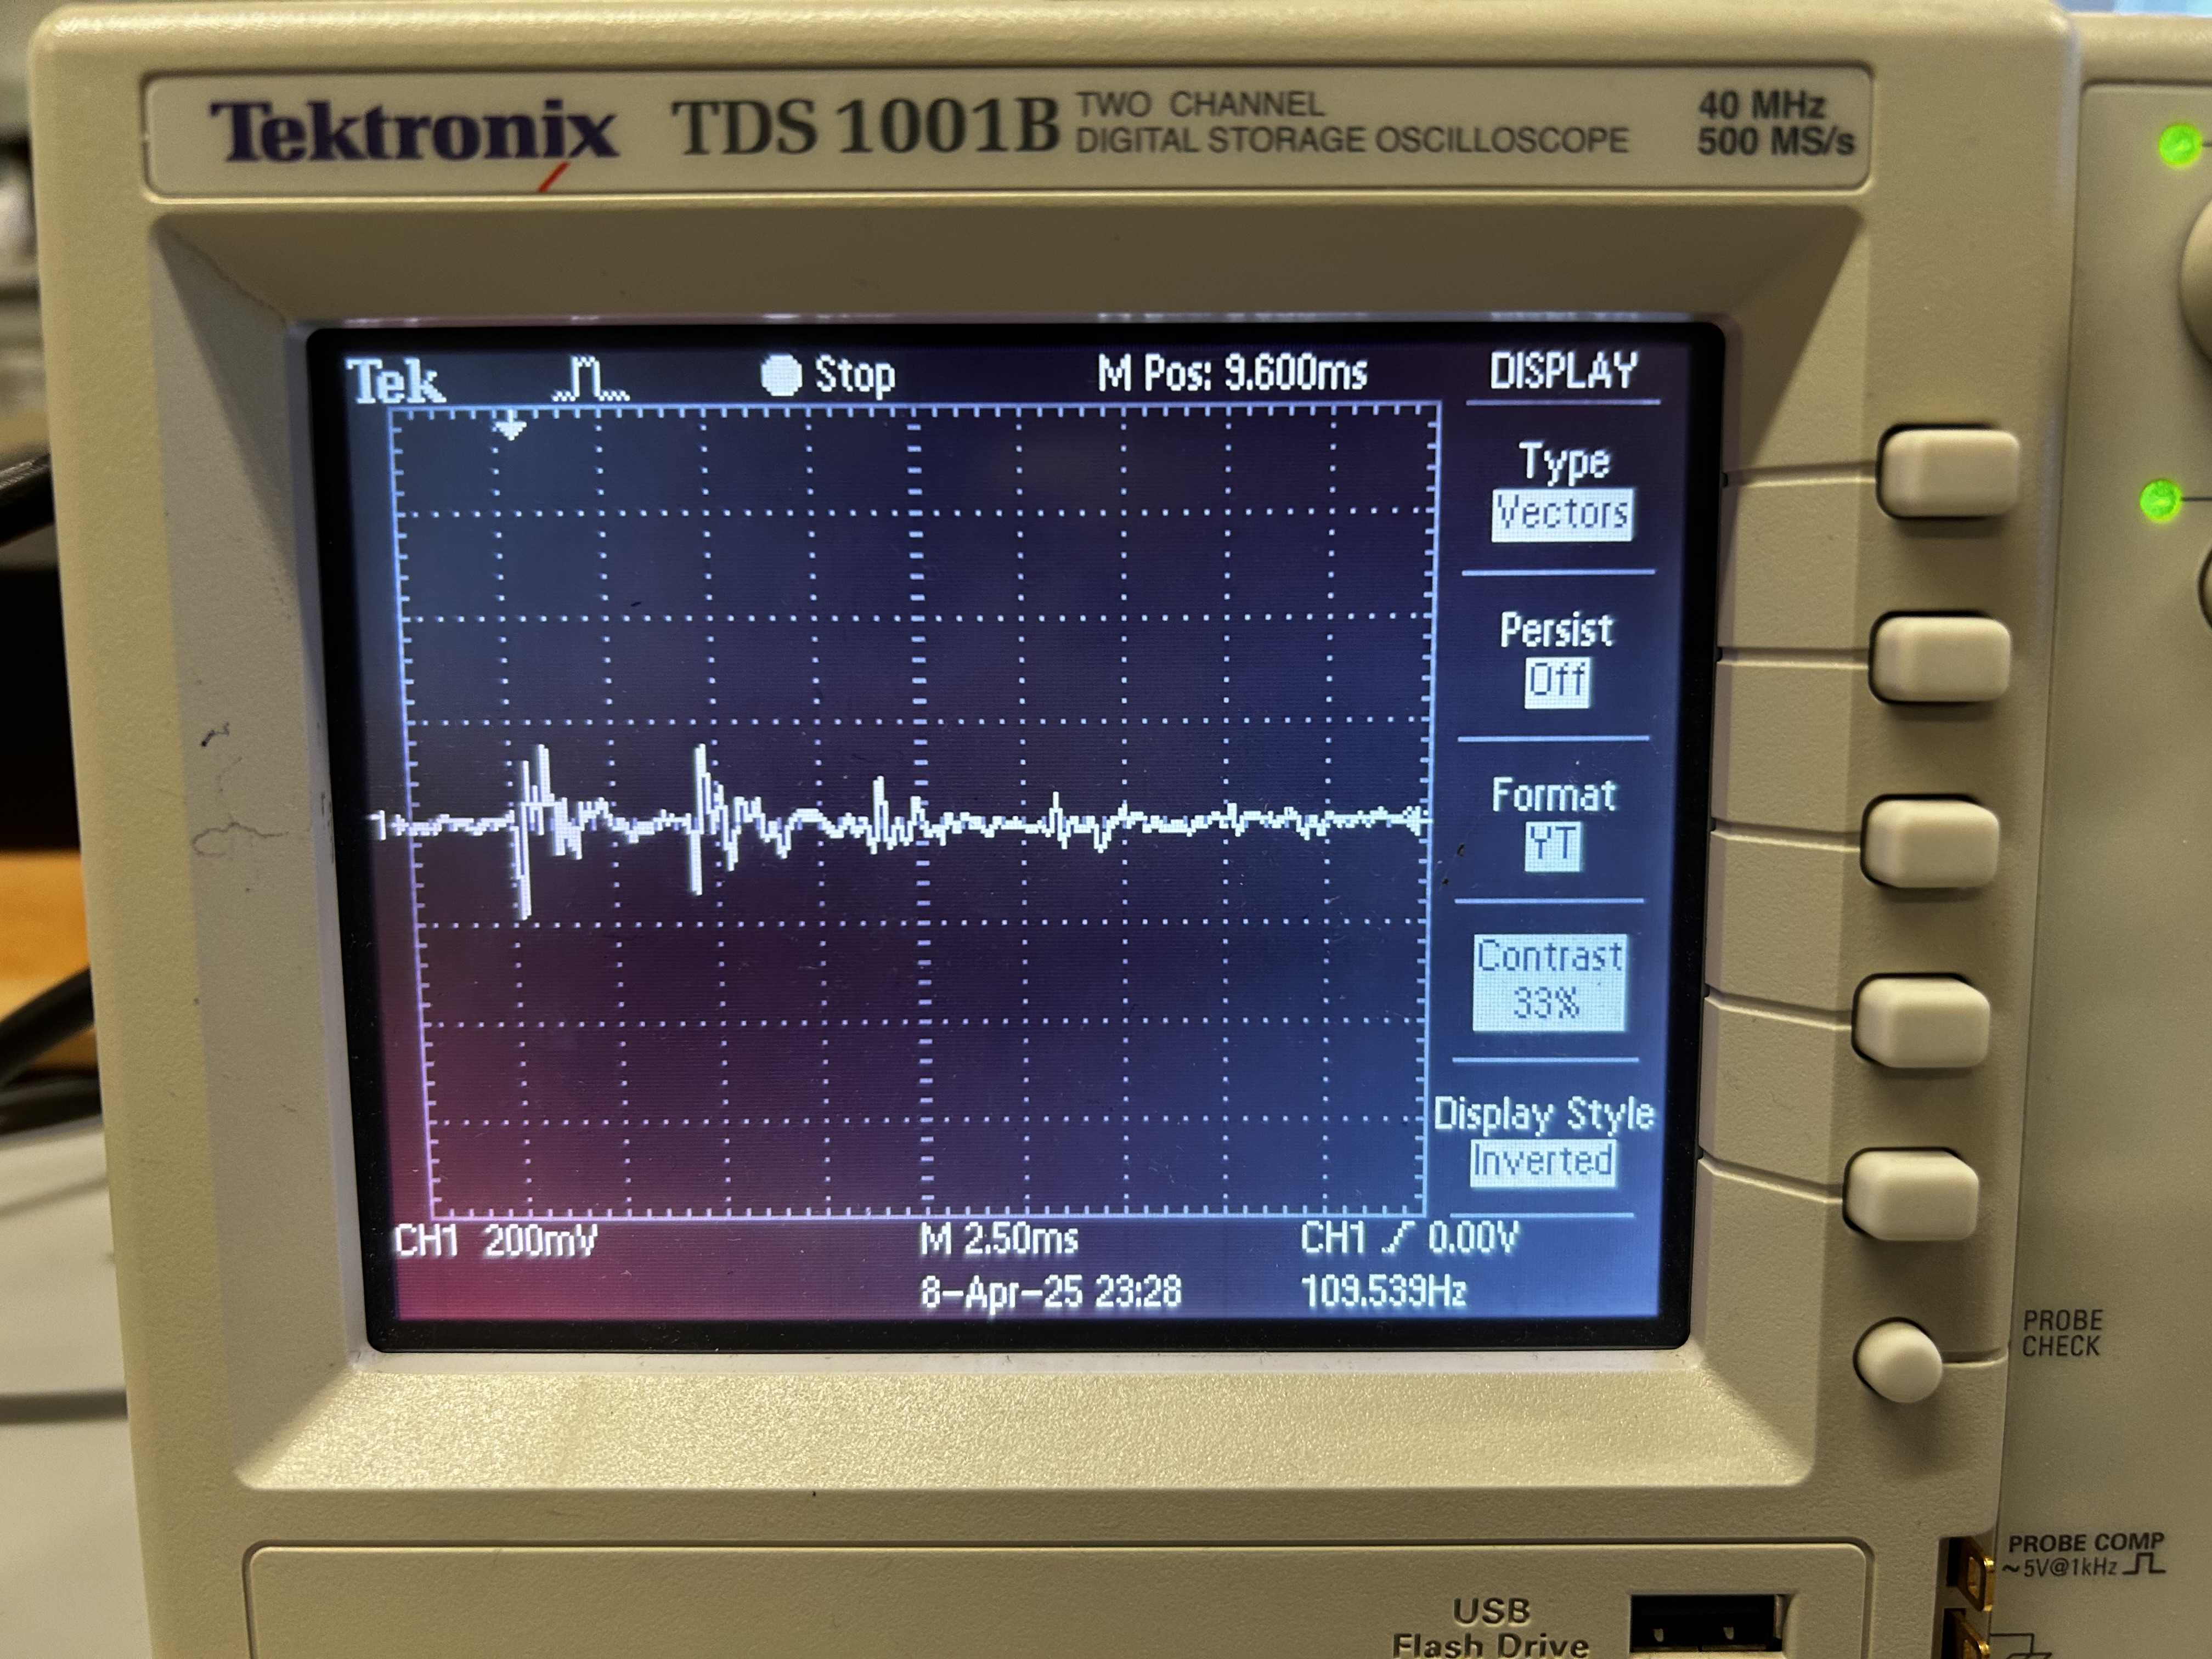
\includegraphics[width=.5\linewidth]{oscil pulses.jpeg}
    \caption{Oscilloscope screen depicting the pulse with echoes.}
    \label{fig:4}
\end{figure}

\section{Results and Discussion} \label{sec:3}

\subsection{Questions: How to Read an Oscilloscope}

\textit{These are answers to the provided questions regarding reading an oscilloscope included in the lab manual.}

\begin{figure}[H]
    \centering
    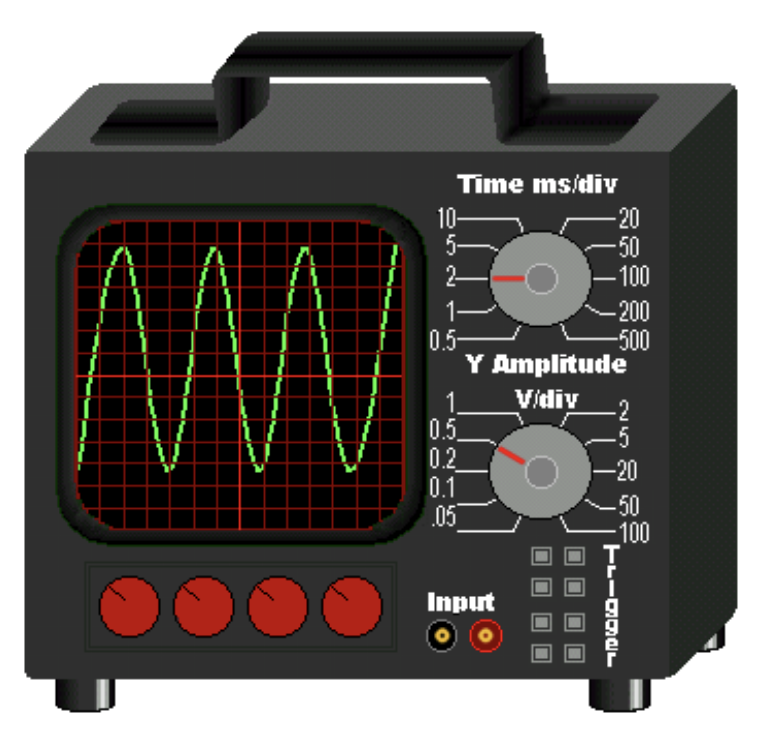
\includegraphics[width=.4\textwidth]{oscil 4 qs.png}
    \caption{Oscilloscope diagram.}
    \label{fig:5}
\end{figure}

\textbf{Q1. What is the period (T) of the wave?}

Seeing the time is set to 2 ms/div, and that there are 8 square divisions that span a peak to another, the period of the wave is \textbf{8 ms}.

\textbf{Q2. What is the peak-to-peak voltage?}

Reading vertically, and noting that the oscilloscope is set to 0.5 V/div, counting 10 square division the peak-to-peak voltage is read to be \textbf{5 V}.

\textbf{Q3. What is the frequency of the signal displayed in the image above?}

\vspace{-2ex}
\begin{gather*}
    f = \frac{1}{T} = \frac{1}{0.008} = \mathbf{125} \: \text{\textbf{HZ}}
\end{gather*}

\subsection{Investigation I}

The results found for this investigation are tabulated in Table \ref{tab:1} below.

\begin{table}[H]
    \centering
    \caption{Table of the results found for different tube length resonances.}
    \label{tab:1}
    \resizebox{.75\textwidth}{!}{%
        \begin{tabular}{|
        >{\columncolor[HTML]{EFEFEF}}c |ccccc|}
        \hline
        \textbf{Frequency (f) (Hz) $\mathbf{\pm 1}$ Hz} & \multicolumn{5}{c|}{\textbf{Piston Positions (L) (cm) $\mathbf{\pm 0.1}$ cm}}                                            \\ \hline
        \textbf{700}                           & \multicolumn{1}{c|}{7.1}  & \multicolumn{1}{c|}{32.2} & \multicolumn{1}{c|}{56.2} & \multicolumn{1}{c|}{82.4} & -    \\ \hline
        \textbf{800}                           & \multicolumn{1}{c|}{11.3} & \multicolumn{1}{c|}{32.9} & \multicolumn{1}{c|}{53.6} & \multicolumn{1}{c|}{60.8} & 74.5 \\ \hline
        \textbf{900}                           & \multicolumn{1}{c|}{4.7}  & \multicolumn{1}{c|}{21.7} & \multicolumn{1}{c|}{41.3} & \multicolumn{1}{c|}{59.9} & 79.2 \\ \hline
        \textbf{1000}                          & \multicolumn{1}{c|}{3.6}  & \multicolumn{1}{c|}{20.2} & \multicolumn{1}{c|}{37.1} & \multicolumn{1}{c|}{54.5} & 71.0 \\ \hline
        \end{tabular}%
    }
\end{table}

To calculate the wavelengths for each n, Eq. \ref{eq:3} was used and the uncertainties for each wavelength were taken with,

\vspace{-2ex}
\begin{gather*}
    \Delta \lambda = \frac{4}{n} \Delta L
\end{gather*}

With the uncertainties for the averages being the standard deviation for the values calculated for each n.

\begin{table}[H]
    \caption{Values calculated for the wavelength with Eq. \ref{eq:3}.}
    \label{tab:3}
    \resizebox{\textwidth}{!}{%
        \begin{tabular}{|
        >{\columncolor[HTML]{EFEFEF}}c |c|c|c|c|}
        \hline
        \textbf{n} & \textbf{700 Hz}         & \textbf{800 Hz}         & \textbf{900 Hz}         & \textbf{1000 Hz}        \\ \hline
        \textbf{1} & 0.2840 m $\pm$ 0.0040 m & 0.4520 m $\pm$ 0.0040 m & 0.1880 m $\pm$ 0.0040 m & 0.1440 m $\pm$ 0.0040 m \\ \hline
        \textbf{3} & 0.4293 m $\pm$ 0.0013 m & 0.4387 m $\pm$ 0.0013 m & 0.2893 m $\pm$ 0.0013 m & 0.2693 m $\pm$ 0.0013 m \\ \hline
        \textbf{5} & 0.4496 m $\pm$ 0.0008 m & 0.4288 m $\pm$ 0.0008 m & 0.3304 m $\pm$ 0.0008 m & 0.2968 m $\pm$ 0.0008 m \\ \hline
        \textbf{7} & 0.4714 m $\pm$ 0.0006 m & 0.3474 m $\pm$ 0.0006 m & 0.3423 m $\pm$ 0.0006 m & 0.3114 m $\pm$ 0.0006 m \\ \hline
        \textbf{9} & -                       & 0.3311 m $\pm$ 0.0004 m & 0.3520 m $\pm$ 0.0004 m & 0.3156 m $\pm$ 0.0004 m \\ \hline\hline
        \textbf{Avg.} &
        \cellcolor[HTML]{EFEFEF}0.4086 m $\pm$ 0.0366 m &
        \cellcolor[HTML]{EFEFEF}0.3996 m $\pm$ 0.0224 m &
        \cellcolor[HTML]{EFEFEF}0.3004 m $\pm$ 0.0269 m &
        \cellcolor[HTML]{EFEFEF}0.2674 m $\pm$ 0.0285 m \\ \hline
        \end{tabular}%
    }
\end{table}

To calculate the speed of sound Eq. \ref{eq:1} was used and the uncertainties for the speed of sound were taken with,

\vspace{-2ex}
\begin{gather*}
    \Delta c = c \: \cdot \: \sqrt{\left( \frac{\Delta f}{f} \right)^2 + \left( \frac{\Delta \lambda}{\lambda} \right)^2}
\end{gather*}

in which the values for $\lambda$ and $\Delta \lambda$ were taken from the averages in Table \ref{tab:3}.

\begin{table}[H]
    \caption{Values calculated for the speed of sound with Eq. \ref{eq:1}.}
    \label{tab:4}
    \resizebox{\textwidth}{!}{%
        \begin{tabular}{|
        >{\columncolor[HTML]{EFEFEF}}c |c|c|c|c|}
        \hline
        \textbf{c = f$\mathbf{\lambda}$} & \textbf{700 Hz}            & \textbf{800 Hz}            & \textbf{900 Hz}            & \textbf{1000 Hz}           \\ \hline
        \textbf{c =}                     & 286.02 m/s $\pm$ 25.62 m/s & 319.68 m/s $\pm$ 17.92 m/s & 270.36 m/s $\pm$ 24.21 m/s & 267.40 m/s $\pm$ 28.50 m/s \\ \hline
        \end{tabular}%
    }
\end{table}

As can be observed from Table \ref{tab:4}, the values found for the speed of sound for each frequency observed are not very close to the speed of sound expected at room temperature, 343 m/s.
This value lies close to the speed of sound found for 800 Hz, but does not quite agree with it. The difference between the value found 700 Hz and the expected value is \textbf{56.98 m/s}, or \textbf{18.12\%}. For 800 Hz the difference is \textbf{23.32 m/s}, or \textbf{7.04\%}.
For 900 Hz the difference is \textbf{72.64 m/s}, or \textbf{23.69\%}. For 1000 Hz the difference is \textbf{75.60 m/s}, or \textbf{24.77\%}. These differences are rather large, indicating issues when measuring.

\subsection{Investigation II}

The results found for this investigation are tabulated in Table \ref{tab:2} below.

\begin{table}[H]
    \centering
    \caption{Table of the results found for square wave sound pulses.}
    \label{tab:2}
    \resizebox{.55\textwidth}{!}{%
        \begin{tabular}{|c|c|}
        \hline
        \textbf{distance (L) (cm) $\mathbf{\pm 0.1}$ cm} & \textbf{$\mathbf{\Delta}$t (ms) $\mathbf{\pm 0.5}$ ms} \\ \hline
        75 & 4.25 \\ \hline
        65 & 3.75 \\ \hline
        55 & 3    \\ \hline
        45 & 2.75 \\ \hline
        35 & 2    \\ \hline
        \end{tabular}%
    }
\end{table}

To calculate the speed of sound for this investigation we have to consider the fact that we have measured the time difference between echoes for \textit{pulses} of sound. Because the source is not continuous, we cannot
say it resonates as the previous investigation did. Hence, use:

\vspace{-2ex}
\begin{gather}
    c = \frac{L}{\Delta t}
\end{gather}

But since the echoes are being measured, that would mean that the sound is getting reflected, so the echo would travel 2 lengths (from the speaker, to the piston, back to the microphone). Hence,
the formula becomes,

\vspace{-2ex}
\begin{gather} \label{eq:5}
    c = \frac{2L}{\Delta t}
\end{gather}

\begin{table}[H]
    \centering
    \caption{Values calculated for the speed of sound with Eq. \ref{eq:5}}
    \label{tab:5}
    \resizebox{.8\textwidth}{!}{%
        \begin{tabular}{|c|c|c|}
        \hline
        \textbf{distance (L) (cm) $\mathbf{\pm 0.1}$ cm} & \textbf{$\mathbf{\Delta}$t (ms) $\mathbf{\pm 0.5}$ ms} & \textbf{c = 2L/$\mathbf{\Delta}$t} \\ \hline
        75 & 4.25 & 352.94 m/s $\pm$ 41.525 m/s \\ \hline
        65 & 3.75 & 346.67 m/s $\pm$ 46.226 m/s \\ \hline
        55 & 3    & 366.67 m/s $\pm$ 61.115 m/s \\ \hline
        45 & 2.75 & 327.27 m/s $\pm$ 59.508 m/s \\ \hline
        35 & 2    & 350.00 m/s $\pm$ 87.506 m/s \\ \hline
        \end{tabular}%
    }
\end{table}

Taking the average of the values in Table \ref{tab:5} above with the standard deviation taken as the uncertainty on the value, the speed of sound for this investigation is found to be
\textbf{348.71 m/s} $\mathbf{\pm}$ \textbf{5.678 m/s} . The expected value for the speed of sound in air at room temperature, being 343 m/s, agrees with this value as it lies within the uncertainty confidence interval.
In fact, the difference between the value calculated and the one expected is \textbf{5.71 m/s}, or \textbf{1.65\%}, which is a very small difference in values.

\section{Conclusion} \label{sec:4}

This experiment was effective in demonstrating two different methods for measuring the speed of sound in air with the use of an oscilloscope.

\textbf{Investigation I} used fixed frequency outputs in a closed tube to produce standing wave resonances, the wavelengths of were then calculated and used to find the speed of sound.
For 700 Hz, the speed of sound was found to be \textbf{286.02 m/s} $\mathbf{\pm}$ \textbf{25.62 m/s}. For 800 Hz \textbf{319.68 m/s} $\mathbf{\pm}$ \textbf{17.92 m/s},
for 900 Hz \textbf{270.36 m/s} $\mathbf{\pm}$ \textbf{24.21 m/s}, and for 1000 Hz \textbf{267.40 m/s} $\mathbf{\pm}$ \textbf{28.50 m/s}. These values were lower than the expected 343 m/s at room temperature, with
the highest deviation from this number being \textbf{24.77\%} for 1000 Hz. Errors in measurements could arise from difficulty in determining the peak resonant amplitude on the oscilloscope display, parallax in reading the tube lengths, and poor
oscilloscope settings for amplification. For future renditions of this investigation, greater precautions could be taken to isolate the experiment as the microphone was found to be incredibly senseitive to surrounding sound. More measurements could be taken for
the experiment as well, or for a greater tube length, as during this rendition the tube length was limited to 80 cm. The piston in the tube was also quite loose, meaning there was likely sound leakage.

\textbf{Investigation II} used square wave sound pulses and time difference between the pulse and first echo to calculate the speed of sound in air. This method produced results of \textbf{348.71 m/s} $\mathbf{\pm}$ \textbf{5.678 m/s} which
is agrees with the expected results of 343 m/s at room temperature. The slightly higher speed results would also indicate a warmer room temperature at time of measurement. Overall, this method of measurement would indicate greater accuracy and be less prone to errors as short sound
pulses are less susceptible to interference with surrounding sounds. Further improvements to this experiment could include ensuring the room is at 20$^{\circ}$C as that is the temperature that the standard 343 m/s speed for sound was measured at. By having the experiment done at the same ambient temperature
there would be greater accuracy when comparing results.

\newpage

%%%%%%%%%%%%%%%%%%%%%%%%%%%%%%%%%%%

\bibliographystyle{IEEEtran}
\bibliography{References} \label{sec:ref}

\vspace{1.5cm}

\listoffigures


\end{document}